%2multibyte Version: 5.50.0.2953 CodePage: 1252

\documentclass[bigger]{beamer}
%%%%%%%%%%%%%%%%%%%%%%%%%%%%%%%%%%%%%%%%%%%%%%%%%%%%%%%%%%%%%%%%%%%%%%%%%%%%%%%%%%%%%%%%%%%%%%%%%%%%%%%%%%%%%%%%%%%%%%%%%%%%%%%%%%%%%%%%%%%%%%%%%%%%%%%%%%%%%%%%%%%%%%%%%%%%%%%%%%%%%%%%%%%%%%%%%%%%%%%%%%%%%%%%%%%%%%%%%%%%%%%%%%%%%%%%%%%%%%%%%%%%%%%%%%%%
\usepackage{amsfonts}
\usepackage{amsmath}
\usepackage{mathpazo}
\usepackage{graphicx}
\usepackage{hyperref}
\usepackage{multimedia}


\usetheme{Madrid}
\usecolortheme{beaver}
\usefonttheme{professionalfonts}
\input{tcilatex}
\setbeamertemplate{navigation symbols}{}
\begin{document}

\title[47-805: Optimization]{Optimization: Methods}
\subtitle{Judd Chapter 4}
\author[David Childers]{David Childers (thanks to Y. Kryukov, K. Judd, and U. Doraszelski)}
\institute[CMU]{CMU, Tepper School of Business}
\date[Mar-22]{March 22, 2022}
\maketitle

\section{Optimization}

\begin{frame}%
%EndExpansion

\frametitle{The Plan}

\begin{itemize}
\item Unconstrained optimization

\begin{itemize}
\item Newton: Univariate \& Multivariate

\item Direction methods

\item Derivative-free methods: golden section \& polytope
\end{itemize}

\item Constrained optimization

\begin{itemize}
\item Penalty function

\item Kuhn-Tucker conditions: \newline
GZ and Active set methods
\end{itemize}

\item Structured Problems

\item Code
\end{itemize}

%TCIMACRO{\TeXButton{EndFrame}{\end{frame}}}%
%BeginExpansion
\end{frame}%

\begin{frame}%
%EndExpansion
\frametitle{General points}

\begin{itemize}
\item Optimization is central to Economics

\begin{itemize}
\item Almost every economic decision is represented as solution to an optimization
problem

\item Selfless behavior: add welfare of others to the objective
\end{itemize}

\item As with nonlinear eq-ns, issue with uniqueness and local solutions

\begin{itemize}
\item Uniqueness $\Leftarrow $ global concavity, or quasi-concavity

\item Local solutions: find all and pick the best
\end{itemize}

\item Solving FOC is viable (Newton method), but:

\begin{itemize}
\item Check SOC to avoid wrong kind of extremum, \newline
or inflection points

\item Newton requires second derivative of objective

\item Value of objective measures quality of current guess
\end{itemize}
\end{itemize}

%TCIMACRO{\TeXButton{EndFrame}{\end{frame}}}%
%BeginExpansion
\end{frame}%
%EndExpansion
%TCIMACRO{\TeXButton{BeginFrame}{\begin{frame}}}%
%BeginExpansion
\begin{frame}%
%EndExpansion
\frametitle{Newton's method -- Univariate}

\begin{equation*}
\min_{x\in \mathbb{R}}f(x)
\end{equation*}%
assume $f(x)$ is $C^{3}$ (3x continuously differentiable).

\begin{itemize}
\item Use Newton's method to solve F.O.C. of the problem.

\item Iterate on:%
\begin{equation*}
x^{k+1}=x^{k}-f^{\prime }(x^{k})/f^{\prime \prime }(x^{k})
\end{equation*}

\item Must check S.O.C. after convergence ($f^{\prime \prime }(x^{k})>0$)

\item Will only find local extrema

\begin{itemize}
\item Need global convexity to find global min

\item Or quasi-convexity: $f^{\prime }(x^{k})=0\Rightarrow f^{\prime \prime
}(x^{k})>0$

\item Otherwise, try different (random) starting values
\end{itemize}

\item Converges quadratically to critical point (under same conditions as last time)
\end{itemize}

%TCIMACRO{\TeXButton{EndFrame}{\end{frame}}}%
%BeginExpansion
\end{frame}%
%EndExpansion

%TCIMACRO{\TeXButton{BeginFrame}{\begin{frame}}}%
%BeginExpansion
\begin{frame}%
%EndExpansion

\frametitle{Multivariate Newton}

$f:\mathbb{R}^{n}\mathbb{\rightarrow R}$, $\in C^{3}$

\begin{itemize}
\item Iterate on:%
\begin{equation*}
x^{k+1}=x^{k}-H(x^{k})^{-1}\nabla f(x^{k})^{\prime }
\end{equation*}%
$\nabla f(x)\in \mathbb{R}^{n}$ -- gradient of $f$ (first derivative)\newline
$H(x^{k})$ -- Hessian of $f$ (second derivative)

\item Stopping rules:

\begin{itemize}
\item If $||x^{k+1}-x^{k}||<\epsilon (1+||x^{k}||)$, go to next point.

\item If $||\nabla f(x^{k})||<\delta (1+|f(x^{k})|)$, stop and report
success; otherwise stop and report failure.

\item $\varepsilon $ and $\delta $ should exceed square root of machine
epsilon.
\end{itemize}

\item Computing Hessian by finite diff. = $n^{2}$ evaluations of $f$
\end{itemize}


\end{frame}%

\begin{frame}%

\frametitle{Direction \& line search method}

A sequence of univariate optimization problems

\begin{enumerate}
\item Compute the search (step) direction $s^{k}$:

\begin{itemize}
\item Coordinate directions: Cycle through unit basis vectors $\left\{
e^{j}\right\} _{j=1}^{n}$.

\item Steepest descent: $s^{k}=-\nabla f(x^{k})^{\prime }$.

\item Newton with line search: $s^{k}=-H(x^{k})^{-1}\nabla f(x^{k})^{\prime
} $.
\end{itemize}

\item Compute the step length $\lambda ^{k}$ from a univariate problem: 
\begin{equation*}
\lambda ^{k}=\arg \min_{\lambda }f(x^{k}+\lambda s^{k}).
\end{equation*}

\item Set $x^{k+1}=x^{k}+\lambda ^{k}s^{k}$.

\item If $||x^{k+1}-x^{k}||<\epsilon (1+||x^{k}||)$, go to step 5; o/w go to
1.

\item If $||\nabla f(x^{k})||<\delta (1+|f(x^{k})|)$, report success; o/w,
failure.
\end{enumerate}
\begin{itemize}
\item Under conditions, can ensure guaranteed convergence to stationary point + comparable rate to Newton
\end{itemize}

\end{frame}%

\begin{frame}%

\frametitle{Advanced direction choice methods}

\textbf{Trust Region} methods: alternative to line search
\begin{itemize}
\item Choose direction $\&$ distance subject to sequence of constraints
\end{itemize}

\textbf{Quasi-Newton} methods:

\begin{itemize}
\item Iteratively update Hessian $H^{k+1}$ instead of computing it

\item Use $H^{k}$, $\nabla f(x^{k+1})$, $\nabla f(x^{k})$, $x^{k+1}$, $x^{k}$

\item Methods: DFP, BFGS, Limited-memory (L-)BFGS 

\begin{itemize}
\item BFGS like Broyden, $O(n^2)$ per update but superlinear rate
\item L-BFGS stores only $m<n$ Broyden updates: $O(nm)$ per iterate
\end{itemize}

\item Hessian does not always to converge to the true one
\end{itemize}

\textbf{Conjugate} gradients

\begin{itemize}
\item Do not compute or store the Hessian

\item Dampen the steepest-descent direction:%
\begin{equation*}
s^{k+1}=-\nabla f(x^{k+1})^{\prime }+\frac{||\nabla f(x^{k+1})||^{2}}{%
||\nabla f(x^{k})||^{2}}s^{k}
\end{equation*}

% \item Analogy: a heavy ball rolling down the slope
% 
% \begin{itemize}
% \item Steepest descent: a cart that cannot turn
% \end{itemize}


\end{itemize}


\end{frame}%

\begin{frame}%

\frametitle{Steepest descent vs. Conjugate gradient}

\scalebox{0.7}{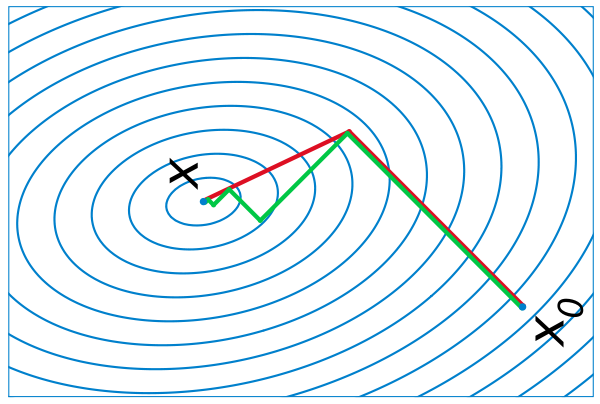
\includegraphics{ConjugateGradientW.png}}



\end{frame}%

\begin{frame}%

\frametitle{Golden section method (univariate)}

Solving $\max_{x}f\left( x\right) $, where $f:\left[ \text{\emph{\b{x}}},%
\bar{x}\right] \rightarrow \mathbb{R}^{1}$ is quasi-concave

\begin{enumerate}
\item Set $A^{0}=$\emph{\b{x}}, $D^{0}=\bar{x}$ (or an interval containing
the max) \newline
$B^{0}=\varphi A^{0}+\left( 1-\varphi \right) D^{0}$, $C^{0}=\left(
1-\varphi \right) A^{0}+\varphi D^{0}$; \newline
evaluate $f_{B}=f\left( B^{0}\right) $, $f_{C}=f(C^{0})$; set $k=0$

\begin{itemize}
\item $\varphi =\left( \sqrt{5}-1\right) /2$ solves $\left( 1-\varphi
\right) /\varphi =\varphi $
\end{itemize}

\item 

\begin{itemize}
\item If $f_{B}>f_{C}$: $A^{k+1}=A^{k}$, $D^{k+1}=C^{k}$, $C^{k+1}=B^{k}$, $%
f_{C}=f_{B}$;\newline
$B^{k+1}=\left( 1-\varphi \right) A^{k+1}+\varphi C^{k+1}$, $f_{B}=f\left(
B^{k+1}\right) $.
\item If $f_{B}<f_{C}$: $A^{k+1}=B^{k}$, $D^{k+1}=D^{k}$, $B^{k+1}=C^{k}$, $%
f_{C}=f_{B}$\newline
$C^{k+1}=\varphi B^{k+1}+\left( 1-\varphi \right) D^{k+1}$, $f_{C}=f\left(
C^{k+1}\right) $
\end{itemize}

\item If $\dfrac{\left\vert D^{k+1}-A^{k+1}\right\vert }{1+\left\vert
B^{k+1}\right\vert }<\delta $, report $B^{k+1}$ as the max
\end{enumerate}

\begin{itemize}
\item Linear convergence at rate $\frac{1}{\varphi}$.
\end{itemize}


\end{frame}%

\begin{frame}%

\frametitle{Polytope (Nelder-Mead, "Amoeba" method) (multivariate)}


Initialization: Choose initial simplex $\{x^{1},\ldots ,x^{n+1}\}$

\begin{enumerate}
\item Reorder vertices such that $f(x^{i})\geq f(x^{i+1})$, $i=1,\ldots ,n$.

\item Find the lowest $i$ such that $f(x^{i})>f(y^{i})$, where 
\begin{equation*}
y^{i}=x^{i}+2\left( \frac{1}{n}\tsum\nolimits_{j\neq i}x^{j}-x^{i}\right)
\end{equation*}%
is the reflection of $x^{i}$ through the opposing face. \newline
If found, set $x^{i}=y^{i}$ and go to step 1; o/w go to step 3.

\item If width of simplex is less than $\varepsilon $, stop; o/w go to step
4.

\item Replace $x^{i}$ with $\frac{1}{2}\left( x^{i}+x^{n+1}\right) $, $%
i=1,\ldots ,n$, i.e., shrink the simplex toward $x^{n+1}$, and go to step 1.
\end{enumerate}

\begin{itemize}
\item Guaranteed to converge to a local minimum if $f$ is continuous.
\end{itemize}


\end{frame}%

\begin{frame}%
%EndExpansion
\frametitle{Constrained optimization}

\begin{equation*}
\begin{array}{cc}
& \min_{x}f(x) \\ 
\text{subject to: } & g(x)=0 \\ 
& h(x)\leq 0%
\end{array}%
\end{equation*}

\begin{itemize}
\item Uniqueness of solution requires:

\begin{itemize}
\item Convexity of objective (concavity for $\max $)

\item Convexity of the feasible set:%
\begin{equation*}
\left\{ x:g(x)=0,h(x)\leq 0\right\}
\end{equation*}%
 e.g. via (quasi-)convexity of $h\left( x\right) $
\end{itemize}

\item Equality constraints could be substituted into objective

\begin{itemize}
\item But (nearly-)linear contraints could be easier to solve \newline
than unconstrained but highly nonlinear problem
\end{itemize}

\item Can pick $f\left( x\right) $ to ensure interior solution
\end{itemize}

\end{frame}

\begin{frame}%

\frametitle{Penalty function method}

Permit anything, but penalize violations: 
\begin{equation*}
\min_{x}f(x)+P\left( \sum_{i}g^{i}(x)^{2}+\sum_{j}\max
(0,h^{j}(x))^{2}\right) ,
\end{equation*}%
where $P>0$ is the penalty parameter. \bigskip

\begin{itemize}
\item Solve repeatedly for an increasing sequence of $P^{k}$'s.

\item Use solution (and Hessian from $P^{k}$) \newline
as the starting point for $P^{k+1}$.

\item Continue until constraint violations are small enough\bigskip

\item Beware limited function domains: $\sqrt{x}$, $\log \left( x\right) $,
etc.
\end{itemize}


\end{frame}%

\begin{frame}%
%EndExpansion

\frametitle{Karush-Kuhn-Tucker Theorem}

\begin{itemize}
\item Define the Lagrangian:%
\begin{equation*}
\mathcal{L}(x,\lambda ,\mu )=f(x)+\lambda ^{T}g(x)+\mu ^{T}h(x)
\end{equation*}

\item Local minimum should satisfy:%
\begin{gather*}
\frac{\partial \mathcal{L}}{\partial x}\equiv f_{x}+\lambda ^{T}g_{x}+\mu
^{T}h_{x}=0 \\
g(x)=0 \\
\mu _{i}h^{i}(x)=0 \\
h^{i}(x)\leq 0,\mu _{i}\geq 0
\end{gather*}

\begin{itemize}
\item Last two lines are called \emph{complementary slackness }conditions
\end{itemize}

\item If binding constraints are linearly independent, $\{\lambda ,\mu \}$
are unique
\end{itemize}

%Describe different constraint qualifications: linear independence is only one possibility



\end{frame}%

\begin{frame}%
%EndExpansion
\frametitle{Solving KKT conditions: brute force}

\begin{itemize}
\item We have no way to solve systems with inequalities in them
\end{itemize}

\textbf{Kuhn-Tucker} approach:

\begin{itemize}
\item $\mathcal{J}=\{1,2,...,m\}$ -- set of all inequality constraints

\item $\mathcal{P\subset J}$ -- set of binding constraints:%
\begin{eqnarray*}
i &\in &\mathcal{P}:h^{i}(x)=0,\mu _{i}\geq 0, \\
i &\not\in &\mathcal{P}:h^{i}(x)\leq 0,\mu _{i}=0,
\end{eqnarray*}
\end{itemize}

\begin{enumerate}
\item Go though for every possible $\mathcal{P}$, \newline
solve equality conditions as a system of equations

\item Drop solutions that violate remaining inequality conditions

\item Report solution with the best objective
\end{enumerate}

Guaranteed to find solution, but computationally intensive


\end{frame}%

\begin{frame}%

\frametitle{Solving KKT: GZ transformation}

\textbf{Zangwil-Garcia} approach:

\begin{enumerate}
\item For every ineqality constraint ($h_{i}(x)\leq 0$), \newline
introduce an unconstrained variable $\xi _{i}$.

\item Replace complementary slackness conditions with:%
\begin{eqnarray*}
h^{i}(x)+[\max \{0,\xi _{i}\}]^{2} &=&0 \\
\mu _{i}-[\max \{0,-\xi _{i}\}]^{2} &=&0
\end{eqnarray*}

\item We have system of equations only

\begin{itemize}
\item And they are differentiable\bigskip
\end{itemize}
\end{enumerate}

\begin{itemize}
\item Can replace $\mu _{i}$ by $[\max \{0,-\xi _{i}\}]^{2}$, reducing \# of
variables
\end{itemize}


\end{frame}%

\begin{frame}%

\frametitle{Active set methods}

Iteratively improve $\mathcal{P}^{k}$ -- set of binding inequality
constraints

\begin{enumerate}
\item Pick initial guess $\mathcal{P}^{0}$

\item Solve using only the constraints in $\mathcal{P}^{k}$, e.g. using
Penalty method

\item Drop constraints that do not bind from $\mathcal{P}^{k}$

\item Add constraints that are violated

\item If no changes in $\mathcal{P}^{k}$, increase the penalty
\end{enumerate}

Linear problem and constraints $\Rightarrow $ \textbf{Simplex }method

\begin{itemize}
\item There must be $n$ binding constraints -- optimum is a vertex of the
feasible set.

\item Replace one constraint at a time, i.e. move from one vertex to
another, along the edges of the facets.

\item Always move in the direction that improves objective
\end{itemize}


\end{frame}%

\begin{frame}%
%EndExpansion

\frametitle{Illustration of Simplex method}


\scalebox{0.25}{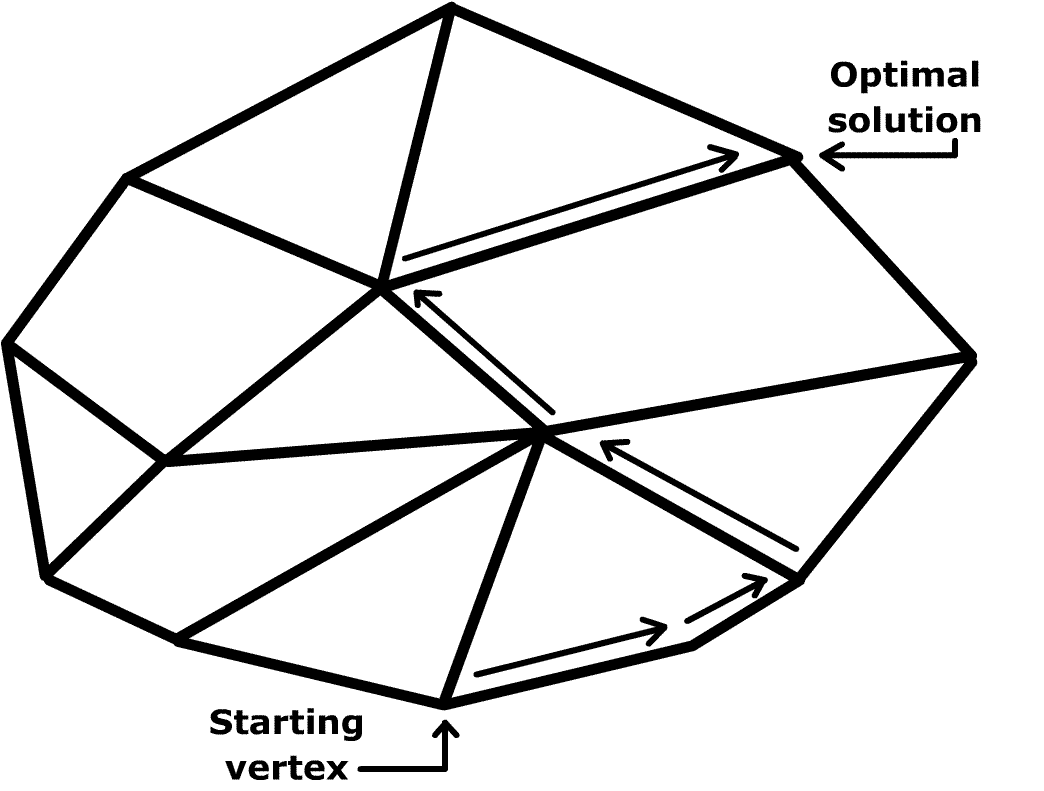
\includegraphics{Simplex_description.png}}

\end{frame}%

\begin{frame}%


\frametitle{Other methods}

\begin{itemize}

\item Interior point methods: like penalization, but \emph{inside} feasible set
\begin{itemize}
\item Provides very strong guarantees for convex problems
\end{itemize}
\item Sequential quadratic programming method: \newline
Replace objective by a quadratic approximation, \newline
and binding constraints by a linear approximation.
\item Reduced gradient method: Use binding constraints to solve for
\textquotedblleft dependent variables\textquotedblright\ in terms of
\textquotedblleft independent variables.\textquotedblright 


\item Randomized methods: useful for avoiding local optima 
\begin{itemize}
\item genetic algorithms, simulated annealing, stochastic gradient descent
\end{itemize}


\end{itemize}


% Add Cost of methods, section on gradient v hessian v no gradient, slide on SGD/ online convex opt? Mention that linear programming exists, is fast? (simplex is polynomial time for "well-conditioned" problems: which are essentially generic, interior point methods ~n^3.5 time in dimension, comparable in practice, a bit more robust).


\end{frame}%

\begin{frame}%

\frametitle{Exploiting Structure}

\begin{itemize}

\item Known structure allows specialized methods, stronger performance

\item \textbf{Linear Programs} Linear objective, linear constraints
\begin{itemize}

\item 0 curvature means Newton (etc) fails, but well known solutions
\item Simplex gives fast exact solutions for well-conditioned problems
\item Interior point methods give $\epsilon$-approx solutions but more robust

\end{itemize}

\item \textbf{Quadratic Programs} Quadratic objective linear constraints
\item \textbf{(Mixed) Integer Programs} Discrete objectives, or mixed discrete and linear or discrete and quadratic
\begin{itemize}
\item Exponentially (NP) hard in general
\item Advanced methods feasible, fast for medium-sized cases
\end{itemize}
\item Structured problems can often be fruitfully combined, and advanced solvers may be able to detect and exploit this

\end{itemize}

\end{frame}

\begin{frame}%

\frametitle{Optimization in Econometrics/Statistics}

\begin{itemize}

\item Econometric problems often have special structure, unique goals
\item (Nonlinear) Least squares/MLE: use information matrix equality
\begin{itemize}
\item Replace Hessian by inner product of Score for 2nd order method
\end{itemize}
\item Due to data randomness, exact optimization not always ideal
\begin{itemize}
\item Randomized or inexact solvers may have \emph{better} performance
\end{itemize}
\item Consider M-estimator: $\hat{\theta}=\underset{\theta\in\Theta}{\arg\min}\frac{1}{n}\sum_{i=1}^{n}m(x_i,\theta)$
\item Stochastic Gradient Descent (Robbins Monro 1951)

\begin{itemize}
\item Choose one data point $x_i$ at random each step
\item Decrease gradient $\theta^{k+1}=\theta^{k}-\lambda^{k}\nabla_\theta m(x_i,\theta^k)$
\item If $\sum_{k=1}^{\infty}\lambda^{k}=\infty$,  $\sum_{k=1}^{\infty}(\lambda^{k})^{2}<\infty$, sequence converges
\item n times faster per step, so ideal for big data and deep learning
\item Many helpful variants and step-size selection methods exist
\end{itemize}




\end{itemize}

\end{frame}

\begin{frame}%

\frametitle{Python solvers: \texttt{scipy.optimize}}

\textbf{Single nonlinear equation} ($f(x)=0$):\newline
\qquad \texttt{root}$\_$\texttt{scalar}\texttt{(lambda x: np.sin(x),x0=3,fprime=lambda x: np.cos(x), method='newton')}

\begin{itemize}

\item \texttt{f} is function, \texttt{lambda x: f(x)} if $f(x)$ defined inline

\item \texttt{fprime}, \texttt{fprime2} take 1st, second derivatives  

\item \texttt{x0} is initial guess: use \texttt{bracket=[a,b]} for bracketing methods

\item \texttt{method} can be \texttt{newton}, \texttt{brentq}, \texttt{secant}, etc 

\end{itemize}


\textbf{System of nonlinear equations}:\newline
\qquad \texttt{root(f,x0,jac=j,method:=hybr)}

\begin{itemize}

\item \texttt{f} is function, \texttt{j} is Jacobian (manual or automatic)
\item \texttt{x0} initial vector
\item \texttt{method} can be \texttt{hybr} (Powell), \texttt{broyden}, \texttt{anderson} (fixed point with acceleration)
\item Options for absolute/relative tolerance, algorithm parameters like acceleration rate, etc

\end{itemize}



\end{frame}%

\begin{frame}%

\frametitle{Python optimizers: \texttt{scipy.optimize} }

\textbf{Univariate optimization}:\newline
\qquad \texttt{minimize}$\_$\texttt{scalar(f,bracket,bounds,method)}
\begin{itemize}
\item Defaults \texttt{bounded} Brent if bounds provided, regular \texttt{Brent} o/w, also \texttt{Golden}
\end{itemize}

\textbf{Multivariate optimization}:\newline
\qquad \texttt{minimize(f,x0,jac,hess,bounds,constraints,method)}
\begin{itemize}
\item Defaults \texttt{BFGS}. Pass jacobian and hessian for first, second order methods, bounds or constraint functions.

\end{itemize}

\textbf{Optimizers for data}
\begin{itemize}
\item \texttt{torch}, \texttt{tensorflow} have SGD and variants (Adam, Adagrad)
\item Use data-loaders to evaluate on small "batch" of data points per iterate
\end{itemize}

%TCIMACRO{\TeXButton{EndFrame}{\end{frame}}}%
%BeginExpansion
\end{frame}%



\begin{frame}%

\frametitle{Julia solvers: \texttt{using Roots, NLsolve}}

\textbf{Single nonlinear equation} ($f(x)=0$):\newline
\qquad \texttt{fzero(x->sin(x),3,order=1)}

\begin{itemize}

\item \texttt{x->f(x)} is $f(x)$ defined inline. Call f for named function

\item \texttt{order} 0 for bisection, 1 for secant 

\item \texttt{3} is initial guess: use \texttt{(a,b)} for bracketing methods

\end{itemize}


\textbf{System of nonlinear equations}:\newline
\qquad \texttt{nlsolve(f,j,x0,method:=trust\_region)}

\begin{itemize}

\item \texttt{f} is function, \texttt{j} is Jacobian (manual or automatic)
\item \texttt{x0} initial vector
\item \texttt{method} can be \texttt{trust\_region}, \texttt{newton} (Newton with linesearch) or \texttt{anderson} (fixed point with acceleration)
\item Options for absolute/relative tolerance, algorithm parameters like acceleration rate, etc

\end{itemize}



\end{frame}%

\begin{frame}%

\frametitle{Julia optimizers: \texttt{using Optim} }

\textbf{Unconstrained optimization}:\newline
\qquad \texttt{optimize(f,g!,h!,x0,Optim.Options)}
\begin{itemize}
\item Defaults \texttt{Brent} if f univariate, \texttt{NelderMead} if no derivatives, \texttt{LBFGS()} if gradient, \texttt{newton} (with line search) if grad \& hessian  
\item \texttt{g!}, \texttt{h!} in-place gradient/hessian, or set \texttt{autodiff:=forward}
\item Also \texttt{ConjugateGradient()}, \texttt{GoldenSection()}, etc

\end{itemize}

\textbf{Constrained optimization}:\newline
\qquad \texttt{df=TwiceDifferentiable(f,g!,h!)}
\qquad \texttt{dc=TwiceDifferentiableConstraints(c,cj!,ch!,lx,lu,lc,uc)}\newline
\qquad \texttt{optimize(df, dc, x0, IPNewton())}

\begin{itemize}
\item minimum of \texttt{f(x)}, subject to $lx\leq x\leq lu$, $lc\leq c(x)\leq uc$

\item Interior Point Newton, using function and constraint derivatives
\end{itemize}

%TCIMACRO{\TeXButton{EndFrame}{\end{frame}}}%
%BeginExpansion
\end{frame}%


\begin{frame}%
%EndExpansion
\frametitle{Implementation: Matlab solvers}

\textbf{Single nonlinear equation} ($f(x)=0$):\newline
\qquad \texttt{X = fzero(@MyFun,3,optimset('Display','iter'))}

\begin{itemize}
\item \texttt{MyFun(x)} is $f(x)$, "\texttt{@}" is function handle operator

\item \texttt{3} is the initial guess (required input)

\item \texttt{optimset} (optional) -- sets parameters:

\begin{itemize}
\item 'Display' = 'iter' means show output for each iteration

\item \texttt{'TolX'=1e-7} is termination tolerance for \newline
$\left\Vert x^{k+1}-x^{k}\right\Vert $ stopping criterion

\item \texttt{'TolFun'} = tolerance for $\left\Vert f(x^{k+1})\right\Vert $
criterion
\end{itemize}

\item \texttt{[x,fval,exitflag] = fsolve(...)}

\begin{itemize}
\item \texttt{fval} -- final value of $f(x)$

\item \texttt{exitflag} = 1 if solution is found, \TEXTsymbol{<} 0 if failed
\end{itemize}

\item Read help for more options
\end{itemize}

%TCIMACRO{\TeXButton{EndFrame}{\end{frame}}}%
%BeginExpansion
\end{frame}%
%EndExpansion
%TCIMACRO{\TeXButton{BeginFrame}{\begin{frame}}}%
%BeginExpansion
\begin{frame}%
%EndExpansion
\frametitle{More Matlab solvers}

\textbf{System of nonlinear equations}:\newline
\qquad \texttt{[x,fval] = fsolve(@myfun,x0,options)}

\begin{itemize}
\item \texttt{function F = myfun (x) }: takes $x$, returns $F(x)$

\item \texttt{myfun }can also compute the Jacobian matrix (read help)
\end{itemize}

\textbf{Unconstrained optimization}:

\begin{itemize}
\item \texttt{fminsearch(@myfun,x0,options)}

\item \texttt{fminunc(@myfun,x0,options)}
\end{itemize}

\textbf{Constrained optimization}:\newline
\qquad \texttt{x = fmincon(@myfun,x0,A,b,Aeq,beq,lb,ub,@mycon)}

\begin{itemize}
\item minimum of \texttt{myfun}, subject to

\item $Ax\leq b$, $A_{eq}x=b_{eq}$

\item $lb\leq x\leq ub$

\item $c(x)\leq 0,c_{eq}(x)=0$ defined by:\newline
\qquad \texttt{function [c,ceq] = mycon(x)}
\end{itemize}

%TCIMACRO{\TeXButton{EndFrame}{\end{frame}}}%
%BeginExpansion
\end{frame}%

\begin{frame}
\frametitle{Conclusions}

\begin{itemize}

\item Generic optimizers exist, but problem knowledge and structure can help immensely

\item Optimization is an active area of computational research.


\item We should take advantage of existing methods and software rather than
developing our own.

\item For serious problems, use structured optimization modeling languages and specialized solvers
\begin{itemize}
\item AMPL or JuMP let you switch out specialized solvers
\item For hard problems like integer programs, solvers like Gurobi millions of times faster
\end{itemize}

\item See code examples in Jupyter notebook



\end{itemize}


\end{frame}


\begin{frame}%
%EndExpansion
\frametitle{Recommended References}

\begin{itemize}

\item General Optimization 
\begin{itemize}
\item Judd Chapter 4.
\item Nocedal, Jorge and Stephen J. Wright. \underline{Numerical Optimization} 2nd ed. 2006
\begin{itemize}
\item Standard reference on classic material, available online
\end{itemize}
\end{itemize}

\item Advanced Methods
\begin{itemize}
\item Ben Tal, Aharon and Arkadi Nemirovski. \underline{Lectures on Modern Convex  Optimization} 2001 \url{https://www2.isye.gatech.edu/~nemirovs/LMCOBookSIAM.pdf}
\item Bubeck, Sebastien. \underline{Convex  Optimization: Algorithms and Complexity} 2015 \url{https://arxiv.org/abs/1405.4980}
\end{itemize}


\item For fun: history and politics of numerical optimization
\begin{itemize}
\item Shalizi, Cosma. "In Soviet Union, Optimization Problem Solves \emph{You}" 2012 \url{http://crookedtimber.org/2012/05/30/in-soviet-union-optimization-problem-solves-you/}
\end{itemize}






\end{itemize}

\end{frame}%

\end{document}
